% Important: If latex complains about unicode characters,
% please use "\usepackage[utf8x]{inputenc}" in your preamble
% You can change the size of the picture by putting it into the construct:
% 1) \resizebox{10cm}{!}{"below picture"} to scale horizontally to 10 cm
% 2) \resizebox{!}{15cm}{"below picture"} to scale vertically to 15 cm
% 3) \resizebox{10cm}{15cm}{"below picture"} a combination of above two
% It is not recomended to use the scale option of the tikzpicture environment.
\resizebox{7cm}{!}{
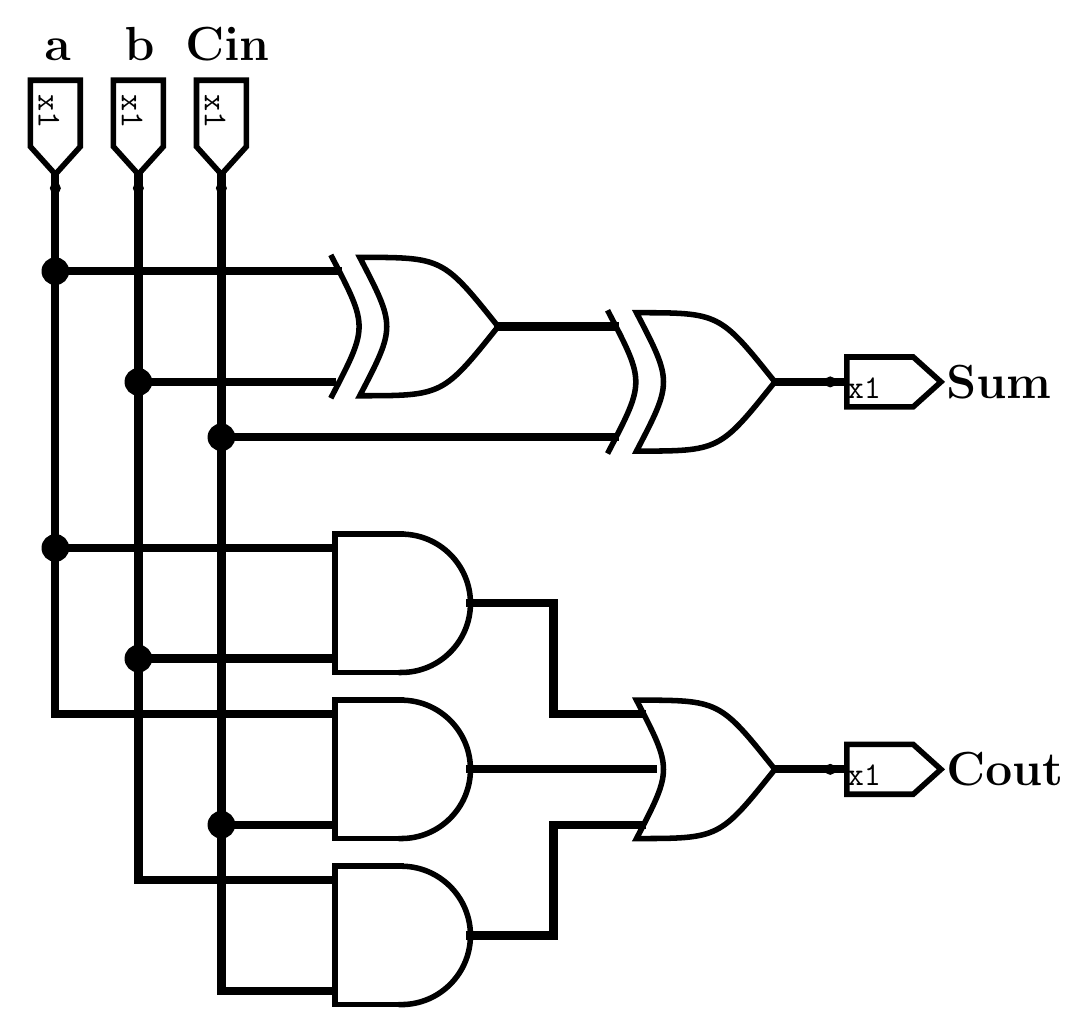
\begin{tikzpicture}[x=1pt,y=-1pt,line cap=rect]
\def\logisimfontA#1{\fontfamily{cmr}{#1}} % Replaced by logisim, original font was "SansSerif"
\def\logisimfontB#1{\fontfamily{cmtt}{#1}} % Replaced by logisim, original font was "Monospaced"
\definecolor{custcol_0_0_0}{RGB}{0, 0, 0}
\definecolor{custcol_ff_ff_ff}{RGB}{255, 255, 255}
\draw [line width=3.0pt, custcol_0_0_0 ]  (15.0,94.0) -- (15.0,194.0) -- (115.0,194.0) ;
\draw [line width=3.0pt, custcol_0_0_0 ]  (275.0,134.0) -- (295.0,134.0) ;
\draw [line width=3.0pt, custcol_0_0_0 ]  (275.0,274.0) -- (295.0,274.0) ;
\draw [line width=3.0pt, custcol_0_0_0 ]  (15.0,194.0) -- (15.0,254.0) -- (115.0,254.0) ;
\draw [line width=3.0pt, custcol_0_0_0 ]  (75.0,294.0) -- (75.0,354.0) -- (115.0,354.0) ;
\draw [line width=3.0pt, custcol_0_0_0 ]  (45.0,234.0) -- (115.0,234.0) ;
\fill [line width=3.0pt, custcol_0_0_0]  (45.0,134.0) ellipse (5.0 and 5.0 );
\fill [line width=3.0pt, custcol_0_0_0]  (15.0,194.0) ellipse (5.0 and 5.0 );
\fill [line width=3.0pt, custcol_0_0_0]  (75.0,154.0) ellipse (5.0 and 5.0 );
\fill [line width=3.0pt, custcol_0_0_0]  (15.0,94.0) ellipse (5.0 and 5.0 );
\fill [line width=3.0pt, custcol_0_0_0]  (75.0,294.0) ellipse (5.0 and 5.0 );
\fill [line width=3.0pt, custcol_0_0_0]  (45.0,234.0) ellipse (5.0 and 5.0 );
\draw [line width=3.0pt, custcol_0_0_0 ]  (75.0,59.0) -- (75.0,64.0) -- (75.0,154.0) -- (75.0,294.0) -- (115.0,294.0) ;
\draw [line width=2.0pt, custcol_0_0_0 ]  (66.0,49.0) -- (75.0,59.0) -- (84.0,49.0) -- (84.0,25.0) -- (66.0,25.0) -- cycle;
\logisimfontB{\fontsize{12pt}{12pt}\selectfont\node[inner sep=0, outer sep=0, custcol_0_0_0, anchor=base west, rotate=-90.0] at  (69.0,30.0)  {x1};}
\logisimfontA{\fontsize{16pt}{16pt}\fontseries{bx}\selectfont\node[inner sep=0, outer sep=0, custcol_0_0_0, anchor=base west] at  (62.0,18.0)  {Cin};}
\fill [line width=2.0pt, custcol_0_0_0]  (75.0,64.0) ellipse (2.0 and 2.0 );
\draw [line width=2.0pt, custcol_0_0_0 ]  (6.0,49.0) -- (15.0,59.0) -- (24.0,49.0) -- (24.0,25.0) -- (6.0,25.0) -- cycle;
\logisimfontB{\fontsize{12pt}{12pt}\selectfont\node[inner sep=0, outer sep=0, custcol_0_0_0, anchor=base west, rotate=-90.0] at  (9.0,30.0)  {x1};}
\logisimfontA{\fontsize{16pt}{16pt}\fontseries{bx}\selectfont\node[inner sep=0, outer sep=0, custcol_0_0_0, anchor=base west] at  (11.0,18.0)  {a};}
\fill [line width=2.0pt, custcol_0_0_0]  (15.0,64.0) ellipse (2.0 and 2.0 );
\draw [line width=2.0pt, custcol_0_0_0] (140.0,359.0) arc (90.0:-90.0:25.0 and 25.0 );
\draw [line width=2.0pt, custcol_0_0_0 ]  (140.0,309.0) -- (116.0,309.0) -- (116.0,359.0) -- (140.0,359.0) ;
\draw [line width=3.0pt, custcol_0_0_0 ]  (165.0,214.0) -- (195.0,214.0) -- (195.0,254.0) -- (225.0,254.0) -- (227.0,254.0) ;
\draw [line width=3.0pt, custcol_0_0_0 ]  (165.0,274.0) -- (225.0,274.0) -- (231.0,274.0) ;
\draw [line width=3.0pt, custcol_0_0_0 ]  (165.0,334.0) -- (195.0,334.0) -- (195.0,294.0) -- (225.0,294.0) -- (227.0,294.0) ;
\draw [line width=2.0pt, custcol_0_0_0 ]  (275.0,274.0) .. controls  (255.0,249.0)  ..  (225.0,249.0) .. controls  (238.0,274.0)  ..  (225.0,299.0) .. controls  (255.0,299.0)  ..  (275.0,274.0) -- cycle ;
\draw [line width=3.0pt, custcol_0_0_0 ]  (175.0,114.0) -- (215.0,114.0) -- (217.0,114.0) ;
\draw [line width=3.0pt, custcol_0_0_0 ]  (75.0,154.0) -- (215.0,154.0) -- (217.0,154.0) ;
\draw [line width=2.0pt, custcol_0_0_0 ]  (275.0,134.0) .. controls  (255.0,109.0)  ..  (225.0,109.0) .. controls  (238.0,134.0)  ..  (225.0,159.0) .. controls  (255.0,159.0)  ..  (275.0,134.0) -- cycle ;
\draw [line width=2.0pt, custcol_0_0_0 ]  (215.0,109.0) .. controls  (228.0,134.0)  ..  (215.0,159.0) ;
\draw [line width=3.0pt, custcol_0_0_0 ]  (299.0,134.0) -- (296.0,134.0) ;
\draw [line width=2.0pt, custcol_0_0_0 ]  (325.0,125.0) -- (335.0,134.0) -- (325.0,143.0) -- (301.0,143.0) -- (301.0,125.0) -- cycle;
\logisimfontB{\fontsize{12pt}{12pt}\selectfont\node[inner sep=0, outer sep=0, custcol_0_0_0, anchor=base west] at  (301.0,140.0)  {x1};}
\logisimfontA{\fontsize{16pt}{16pt}\fontseries{bx}\selectfont\node[inner sep=0, outer sep=0, custcol_0_0_0, anchor=base west] at  (337.0,140.0)  {Sum};}
\fill [line width=2.0pt, custcol_0_0_0]  (295.0,134.0) ellipse (2.0 and 2.0 );
\draw [line width=3.0pt, custcol_0_0_0 ]  (45.0,59.0) -- (45.0,64.0) -- (45.0,134.0) -- (45.0,234.0) -- (45.0,314.0) -- (115.0,314.0) ;
\draw [line width=2.0pt, custcol_0_0_0 ]  (36.0,49.0) -- (45.0,59.0) -- (54.0,49.0) -- (54.0,25.0) -- (36.0,25.0) -- cycle;
\logisimfontB{\fontsize{12pt}{12pt}\selectfont\node[inner sep=0, outer sep=0, custcol_0_0_0, anchor=base west, rotate=-90.0] at  (39.0,30.0)  {x1};}
\logisimfontA{\fontsize{16pt}{16pt}\fontseries{bx}\selectfont\node[inner sep=0, outer sep=0, custcol_0_0_0, anchor=base west] at  (40.0,18.0)  {b};}
\fill [line width=2.0pt, custcol_0_0_0]  (45.0,64.0) ellipse (2.0 and 2.0 );
\draw [line width=2.0pt, custcol_0_0_0] (140.0,299.0) arc (90.0:-90.0:25.0 and 25.0 );
\draw [line width=2.0pt, custcol_0_0_0 ]  (140.0,249.0) -- (116.0,249.0) -- (116.0,299.0) -- (140.0,299.0) ;
\draw [line width=3.0pt, custcol_0_0_0 ]  (299.0,274.0) -- (296.0,274.0) ;
\draw [line width=2.0pt, custcol_0_0_0 ]  (325.0,265.0) -- (335.0,274.0) -- (325.0,283.0) -- (301.0,283.0) -- (301.0,265.0) -- cycle;
\logisimfontB{\fontsize{12pt}{12pt}\selectfont\node[inner sep=0, outer sep=0, custcol_0_0_0, anchor=base west] at  (301.0,280.0)  {x1};}
\logisimfontA{\fontsize{16pt}{16pt}\fontseries{bx}\selectfont\node[inner sep=0, outer sep=0, custcol_0_0_0, anchor=base west] at  (337.0,280.0)  {Cout};}
\fill [line width=2.0pt, custcol_0_0_0]  (295.0,274.0) ellipse (2.0 and 2.0 );
\draw [line width=2.0pt, custcol_0_0_0] (140.0,239.0) arc (90.0:-90.0:25.0 and 25.0 );
\draw [line width=2.0pt, custcol_0_0_0 ]  (140.0,189.0) -- (116.0,189.0) -- (116.0,239.0) -- (140.0,239.0) ;
\draw [line width=3.0pt, custcol_0_0_0 ]  (15.0,59.0) -- (15.0,64.0) -- (15.0,94.0) -- (115.0,94.0) -- (117.0,94.0) ;
\draw [line width=3.0pt, custcol_0_0_0 ]  (45.0,134.0) -- (115.0,134.0) -- (115.0,134.0) ;
\draw [line width=2.0pt, custcol_0_0_0 ]  (175.0,114.0) .. controls  (155.0,89.0)  ..  (125.0,89.0) .. controls  (138.0,114.0)  ..  (125.0,139.0) .. controls  (155.0,139.0)  ..  (175.0,114.0) -- cycle ;
\draw [line width=2.0pt, custcol_0_0_0 ]  (115.0,89.0) .. controls  (128.0,114.0)  ..  (115.0,139.0) ;
\end{tikzpicture}
}
